\documentclass[10pt]{article}
\usepackage[margin=0.85in]{geometry}
\usepackage{amsmath,amssymb,amsthm}
\usepackage[hidelinks]{hyperref}
\usepackage{tikz}
\usetikzlibrary{arrows.meta}

\newtheorem{theorem}{Theorem}
\newtheorem{lemma}[theorem]{Lemma}
\newtheorem{proposition}[theorem]{Proposition}
\newcommand{\pk}{\mathsf{pk}}
\newcommand{\sk}{\mathsf{sk}}
\newcommand{\Ent}{\mathsf{H}}
\newcommand{\KL}{\mathsf{D}}
\newcommand{\pos}[1]{\left[#1\right]_+}

\title{A Verification Lower Bound for Hash-Based One-Time Signatures}
\author{}
\date{}

\begin{document}
\maketitle

\begin{abstract}
We study the verification cost of graph-based hash-based one-time signatures with one bare random oracle on bit strings. The model provides no labels, tweaks, or domain separation. With a 128-bit public key, signatures of at most 5504 bits, a 1024-compression key-generation budget, and the stated 127-bit security requirement, every weakly secure scheme has a signature costing at least 18 compressions to verify. A concrete strongly secure scheme verifies every signature in 104. Both bounds are proved in Lean and accepted by the official verifier. The lower proof uses repeated reconstruction patterns and fresh message domains in the actual oracle cache. We also exhibit counterexamples to the proposed fresh-coordinate entropy lemmas used to suggest a bare-oracle lower bound of 24.
\end{abstract}

\setcounter{tocdepth}{2}
\tableofcontents

\section{Introduction}\label{sec:intro}

A graph-based one-time signature reveals values of a fixed computation on secret random inputs. Verification reconstructs the root hash and compares its 128-bit prefix with the public key. We count one compression for each started 512-bit block of a hash input, with a minimum charge of one. Other computation and private randomness are free.

The oracle accepts only a bit string, including its length. Equal strings at different graph nodes receive the same answer. A graph query can also equal the message-and-nonce query that chooses the disclosure index. A lower bound must cover these cases without imposing any separation condition on the scheme.

\paragraph{Verified bounds.}
The lower certificate establishes 18 compressions for every weakly secure scheme, without any condition on its hash inputs. The strongly secure upper certificate establishes 104 (Section~\ref{sec:scheme} describes the 106-compression forest and its six-subtree variant at 104). Sections~\ref{sec:patterns}--\ref{sec:attack} prove the lower bound using reconstruction patterns and the bare oracle's cache. No lower bound of 24 or 25 is claimed for this model.

\paragraph{Proof idea for 18.}
If every verification costs at most 17, it evaluates at most 15 nonroot hash nodes. Key generation evaluates at most 1024 hash nodes, giving fewer than $2^{110}$ possible reconstruction patterns. There are $2^{115}$ disclosure indices, so at least three quarters of the indices share their pattern with at least seven other indices. An honest signature can be converted to any disclosure with the same pattern without another node query: an algebraic candidate consistent with the observations makes exactly the already checked queries.

It remains to select a target index for a new message. We use the actual lazy-oracle cache. A cache of $b$ strings can intersect the nonce domains of at most $b$ messages. Uniformly sampled 256-bit messages therefore have entirely fresh nonce domains with overwhelming probability, even when the graph uses arbitrary bare strings. Exact signing and nonce-search calculations then give a weak forgery probability at least $9/200$, at cost below $2^{127}/25$.

The old argument using one independent oracle table per hash node does not extend just by changing notation. Appendix~\ref{sec:obstructions} gives exact counterexamples both to a Bell-number correction of the information bound and to the suggested fresh-coordinate construction bound.

\section{Model and verified result}\label{sec:model}

\subsection{One oracle and its cost}

For every finite bit string $u$, the random oracle assigns an independent uniform 256-bit value $H(u)$. Strings of different lengths are different inputs. Repeated inputs receive the cached answer. A query costs
\[
c(u)=\max\left\{1,\left\lceil\frac{|u|}{512}\right\rceil\right\}.
\]
There is no free metadata on a query. A scheme can prepend a tweak using a deterministic node, but those bits are part of its input and its cost. The charge concerns input blocks only, without an additional padding or output charge. Computation, storage, and private uniform sampling are free for all parties.

A public finite DAG has source, deterministic, and hash nodes; each node $v$ has a fixed output length $b_v$. Sources contain independent uniform strings of prescribed lengths. A deterministic node applies any public oracle-free function of its declared parents; it can also produce a constant. A hash node has one parent and returns $H$ of the parent's value. Its output has length 256. Parents precede children in a fixed topological order. Input lengths can be zero.

The distinguished root $r$ is a hash node. There need not be a unique sink, and some nodes may have no path to the root. The graph and its functions are fixed independently of the oracle. In particular, no injectivity, tagging, collision-freedom, or other side condition is imposed on its queries.

Key generation samples the sources and evaluates all nodes. If $I_g$ is the input of hash node $g$, its fixed cost is $c_g=c(I_g)$. Write $Z$ for all source strings and $Y_g=H(I_g)$ for the hash outputs. The record $(Z,(Y_g)_g)$ determines all node values by deterministic evaluation. These outputs need not be independent. The public key is the low 128 bits of the root output, matching \texttt{BitVec.setWidth} in the contract. Key generation costs $\sum_g c_g\le1024$.

\subsection{Disclosure and reconstruction}

The scheme specifies $M=2^{115}$ disclosure sets $A_i$. Each excludes $r$ and meets every source-to-root path. The values disclosed at $A_i$, in node order, occupy
\[
\ell_i=\sum_{v\in A_i}b_v\le5376
\]
bits. Sets may coincide. Reconstruction walks backward from the root, stopping at disclosed nodes, and evaluates all other visited nodes in topological order. Let $E_i$ be its hash nodes. Both $E_i$ and its cost are fixed by the graph and the index. The cut condition ensures that no undisclosed source is evaluated. Honest reconstruction repeats the corresponding key-generation queries and returns the honest root, irrespective of query collisions.

\subsection{Signing, verification, and security}

For 256-bit messages and 128-bit nonces, set
\[
\mathsf{idx}(m,\eta)=\operatorname{low}_{128}H(m\Vert\eta).
\]
This query costs one compression. Signing samples fresh nonces without replacement until the index is below $M$, returning the nonce and the values at that disclosure set; it gives up after $L=2^{20}$ trials. Verification queries the same index, checks the revealed length, reconstructs the root, and compares its low 128 bits with the public key. Thus
\[
|\sigma|=128+\ell_i\le5504,\qquad
C_i=1+\sum_{g\in E_i}c_g.
\]
In this model the index query is not automatically independent of key generation. Section~\ref{sec:fresh} proves the independence needed by the attack, directly from fresh cache entries.

An attacker receives the public key, requests one signature, and outputs a message--signature pair. Strong unforgeability counts any accepted pair different from the signed pair; weak unforgeability requires a different message. If signing fails, any accepted pair counts. For every adversary whose complete experiment costs at most $B$ on every execution path, security requires
\begin{equation}\label{eq:security}
\Pr[\mathrm{Forge}]<B/2^{127}.
\end{equation}
The cost includes key generation, signing, all attacker queries, and final verification. The public challenge statements use strong security. The lower-bound theorem below also covers weakly secure schemes because its forgery changes the message.

\begin{theorem}[Verification lower bound]\label{thm:main}
Every weakly secure scheme with these parameters has $\max_i C_i\ge18$. The same conclusion holds for every strongly secure scheme.
\end{theorem}

The proof is completed in Section~\ref{sec:attack}. The elementary observation $C_i\ge2$ holds for every scheme without any security hypothesis: the index query costs one compression, and the root is a hash node that is never disclosed and is always reconstructed. The stronger bound uses weak security to exclude the attack constructed below.

\section{Counting reconstruction patterns}\label{sec:patterns}

Assume for contradiction that every $C_i\le17$. Write
\[
V_i=E_i\setminus\{r\},\qquad
[i]=\{j:E_j=E_i\}.
\]
Every hash costs at least one compression. The index and root account for two, so $|V_i|\le15$. Key generation contains at most 1024 hash nodes, leaving at most 1023 nonroot hash nodes.

\begin{lemma}[Pattern count]\label{lem:patterns}
There are fewer than $2^{110}$ distinct sets $V_i$. At least three quarters of the $M$ indices have $|[i]|\ge8$.
\end{lemma}
\begin{proof}
The number of subsets of size at most 15 of a 1023-element universe is
\begin{equation}\label{eq:pattern-count}
N_* = \sum_{k=0}^{15}\binom{1023}{k}<2^{110}.
\end{equation}
The exact integer inequality is certified in \texttt{Patterns.lean}. A class of size below eight contributes at most seven indices, hence certainly at most eight. Thus the number of indices in such classes is at most $8N_*\le2^{113}=M/4$.
\end{proof}

This count concerns syntactic hash-node sets. It does not assume different nodes make different queries, or that disclosure sets themselves are distinct. Because the root lies in every $E_i$, equality of the sets $V_i$ is exactly equality of the sets $E_i$.

\section{Conversion between equal patterns}\label{sec:conversion}

Fix an honest disclosure at index $i$. Query its index and reconstruct it, retaining the revealed values $x$ and the reconstructed hash outputs $y=(y_g)_{g\in E_i}$. An algebraic record assigns arbitrary source strings and arbitrary 256-bit values to hash nodes; deterministic evaluation then supplies every other value. Such a record need not correspond to a globally consistent bare oracle.

Let
\[
\mathcal C=\{\xi:X_{A_i}(\xi)=x\text{ and }Y_g(\xi)=y_g\text{ for all }g\in E_i\}.
\]
This finite set is enumerable with free computation and contains the actual key-generation record. Choose any member $\xi'$, without any claim about the posterior distribution of actual records.

\begin{lemma}[Cached conversion]\label{lem:conversion}
For every $j$ with $E_j\subseteq E_i$, revealing $X_{A_j}(\xi')$ reconstructs the honest root. Every target hash query already has its required answer in the cache after the honest reconstruction.
\end{lemma}
\begin{proof}
First compare the evaluation of $\xi'$ with the honest reconstruction at $i$. Revealed values agree by definition. Deterministic nodes agree when their parents agree. Hash outputs in $E_i$ agree by the definition of $\mathcal C$. Induction proves agreement at every visited node, including the parent input of every hash in $E_i$. Thus each candidate pair $(I_g(\xi'),Y_g(\xi'))$ for $g\in E_i$ is exactly an observed, cached oracle pair.

Now reconstruct at $j$ using the candidate's disclosed values. At a deterministic node, agreement follows from parent agreement. Each reconstructed hash belongs to $E_j\subseteq E_i$ and therefore has the candidate's cached answer. The resulting root is the candidate root, which equals the observed honest root because the root belongs to $E_i$. Repeated inputs cause no problem: every pair actually queried is already in the single consistent cache.
\end{proof}

Construction of the new disclosure makes no oracle queries. Final verification still pays its specified query cost, including queries that hit the cache. \texttt{Conversion.lean} proves the transfer using cache consistency from actual key generation, rather than an assumption that a family of node-indexed tables is independent.

\section{Fresh messages, signing, and nonce search}\label{sec:fresh}

A message $m$ is \emph{fresh for a cache} $c$ if every input $m\Vert\eta$ is absent from $c$. These message domains are disjoint. A cache supported on a set $D$ of queries can therefore make at most $|D|$ messages nonfresh: assign each offending message the high 256 bits of a cached 384-bit string. Queries of other lengths cannot witness an intersection.

\begin{lemma}[Fresh message mass]\label{lem:fresh}
A uniformly sampled message is fresh with probability at least $1-|D|/2^{256}$. Requiring it also to differ from one specified message lowers this bound by at most $2^{-256}$. In particular both bounds exceed $9/10$ when $|D|\le2^{22}$.
\end{lemma}
\begin{proof}
There are at most $|D|$ excluded prefixes, or $|D|+1$ after excluding the specified message. Divide these counts by $2^{256}$. A computation of cost at most $b$ adds at most $b$ cache entries, since each hash query costs at least one and uniform sampling adds none.
\end{proof}

This statement holds for every fixed current cache, regardless of how it was obtained. Conditioning on that cache requires no independence between graph inputs and past queries.

\begin{lemma}[Signing at a fresh message]\label{lem:signing}
Let $G\subseteq\{0,\ldots,M-1\}$. If the message is fresh at the start of signing, the probability of returning an index in $G$ within $k$ trials is
\begin{equation}\label{eq:signing}
\frac{|G|}{M}\left(1-\left(1-\frac{M}{2^{128}}\right)^k\right),
\end{equation}
provided at least $k$ untried nonces remain. For $k=L$ and $|G|\ge3M/4$, this probability is at least $1/2$.
\end{lemma}
\begin{proof}
Each trial queries a new string and returns a uniform 128-bit index. An invalid answer has probability $1-M/2^{128}$ and leaves every untried nonce input fresh. Thus the probability of landing in $G$ obeys $s_0=0$ and
\[
s_{k+1}=|G|/2^{128}+(1-M/2^{128})s_k,
\]
which gives~\eqref{eq:signing}. This is a direct induction on the signing loop and its cache in \texttt{SignFresh.lean}.

For $0\le p\le1$,
\begin{equation}\label{eq:reciprocal}
(1-p)^k\le\frac1{1+kp}.
\end{equation}
Indeed $(1+kp)(1-p)^k\le1$ by induction, using
$(1+(k+1)p)(1-p)\le1+kp$. Here $p=2^{-13}$ and $k=2^{20}$, so the failure probability is at most $1/129$. The probability in~\eqref{eq:signing} is therefore at least $96/129>1/2$.
\end{proof}

\begin{lemma}[Searching a fresh message]\label{lem:search}
For a fresh message, $T=2^{122}$ distinct nonce queries hit a fixed set of at least eight valid indices with probability at least $1/9$.
\end{lemma}
\begin{proof}
The failure probability is $(1-|G|/2^{128})^T$. It is at most the failure probability for any eight-element subset of $G$, and~\eqref{eq:reciprocal} bounds the latter by
\[
\frac1{1+T\cdot8/2^{128}}=\frac89.
\]
There are enough nonces since $T<2^{128}$.
\end{proof}

\section{The lower bound of 18}\label{sec:attack}

We now assemble the attack in the single-oracle experiment and prove Theorem~\ref{thm:main}.

\begin{proof}[Proof of Theorem~\ref{thm:main}]
Suppose every $C_i\le17$. The attacker performs the following steps.
\begin{enumerate}
\item After key generation, sample a uniform message $m_1$ and request its signature.
\item If signing succeeds at index $i$, reconstruct the signed disclosure. This repeats key-generation queries and leaves the cache unchanged. If signing fails, return a deliberately invalid-length signature.
\item Sample another uniform message $m_2$ after signing and reconstruction. If $m_2=m_1$, return an invalid-length signature. Otherwise search $T=2^{122}$ distinct nonces for an index $j\in[i]$.
\item If the search succeeds, return the converted disclosure of Lemma~\ref{lem:conversion} at $j$. Otherwise return an invalid-length signature.
\end{enumerate}
Freshness is an analysis event, not a test the attacker must perform. An invalid-length fallback always fails verification, so its arbitrary values do not affect the lower success estimate.

Key generation leaves at most 1024 cached strings. By Lemma~\ref{lem:fresh}, $m_1$ is fresh with probability at least $9/10$. Conditional on any such message and any key-generation cache, Lemmas~\ref{lem:patterns} and~\ref{lem:signing} give probability at least $1/2$ of signing at an index $i$ with $|[i]|\ge8$.

Signing adds at most $L$ cache entries. The honest reconstruction adds none, so before sampling $m_2$ the cache has at most $1024+L<2^{22}$ entries. Conditional on every history just described, $m_2$ is fresh and different from $m_1$ with probability at least $9/10$. Lemma~\ref{lem:search} then gives success at least $1/9$. Cached conversion makes the final verifier accept, and the message is new. Applying these bounds successively to conditional probabilities gives
\begin{equation}\label{eq:success}
\Pr[\mathrm{WeakForge}]\ge\frac9{10}\cdot\frac12\cdot\frac9{10}\cdot\frac19
=\frac9{200}.
\end{equation}
This calculation takes place entirely in the bare lazy-oracle experiment; there is no auxiliary separated oracle or identical-until-bad error term.

Every path has total cost at most
\begin{equation}\label{eq:budget}
B=1024+2^{20}+2^{122}+2\cdot16+2
=2^{122}+2^{20}+1058.
\end{equation}
The last two units are the attacker's check of the signed index and the final verifier's index query; the two terms of size 16 cover the honest and final reconstruction. Nonce search costs at most $T$. Exact integer arithmetic gives
\[
B/2^{127}<1/25<9/200,
\]
contradicting weak security.
\end{proof}

\paragraph{Scope and limitations.}
No step restricts the scheme's hash strings. The argument tolerates repeated node queries, node/index collisions outside the favorable freshness events, arbitrary deterministic functions, repeated disclosure sets, and nodes that do not reach the root. It uses no bound on the signature length beyond the original contract and the invalid-length fallback. At 16 nonroot hash nodes, the pattern count is already larger than $2^{115}$, so this particular argument does not prove 19. Bounds of 24 or 25 require a different argument; the counterexamples below rule out the suggested direct entropy port, not those bounds themselves.

\section{A concrete scheme}\label{sec:scheme}

This section describes a concrete scheme within the model of Section~\ref{sec:model}. Every signature verifies in 106 compressions, and the scheme meets the security requirement~\eqref{eq:security}.

\subsection{Construction}

The scheme hangs 63 hash chains under a tree of two grouping levels and a root. A signature reveals one value on every path from a secret source to the root, and the disclosure sets are all such cuts of equal verification cost.

\paragraph{The computation.}
For $k=1,\dots,63$ there is a secret source $z_k$ of 128 bits; write $c_{k,0}=z_k$. For $t=1,\dots,14$ the node $c_{k,t}$ holds the low 128 bits of
\[
H(t_{k,t}\Vert c_{k,t-1}).
\]
For $j=1,\dots,21$ the node $g_j$ holds the low 128 bits of $H(t_{g_j}\Vert c_{3j-2,14}\Vert c_{3j-1,14}\Vert c_{3j,14})$, and for $l=1,\dots,7$ the node $e_l$ holds the low 128 bits of $H(t_{e_l}\Vert g_{3l-2}\Vert g_{3l-1}\Vert g_{3l})$. The root is $r=H(t_r\Vert e_1\Vert\cdots\Vert e_7)$, and the public key is its low 128 bits. Each $t_v$ is a distinct 16-bit constant identifying its hash node; the formal scheme uses its graph index. These tweaks are actual input bits produced by deterministic nodes. All prefixes mentioned in this section are the low 128 bits, as in the contract.

Figure~\ref{fig:scheme} shows the shape of the computation and of one signature. Each node of the tree therefore has three children, except the root, which has seven. Including the tweak, a chain hash absorbs 144 bits and a grouping hash 400 bits, so both cost one compression; the root absorbs 912 bits and costs two compressions. None has the 384-bit input length used for index queries. This separation is a property of this particular construction, not a condition in the model or in the lower bound.


\begin{figure}[t]
\centering
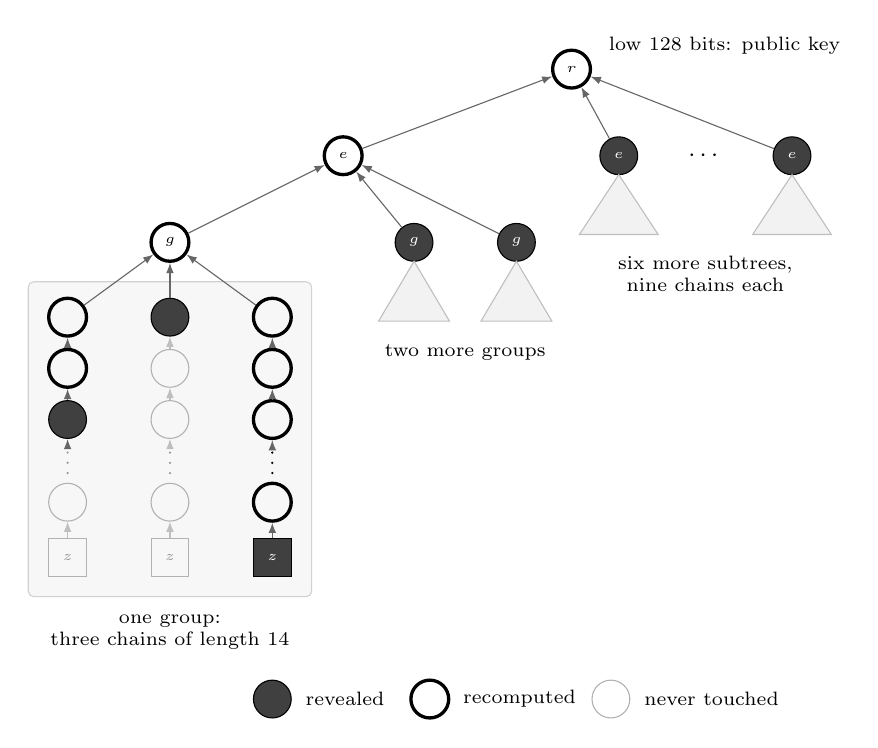
\begin{tikzpicture}[x=1cm,y=1cm,
  v/.style={circle,draw,minimum size=4.8mm,inner sep=0pt,font=\tiny},
  sq/.style={rectangle,draw,minimum size=4.8mm,inner sep=0pt,font=\tiny},
  rev/.style={fill=black!75,text=white},
  hid/.style={draw=black!30,text=black!40},
  ev/.style={very thick},
  a/.style={-{Latex[length=1.3mm]},draw=black!60},
  ah/.style={-{Latex[length=1.3mm]},draw=black!25},
  note/.style={font=\scriptsize,align=center}]

\draw[rounded corners=2pt,draw=black!18,fill=black!3] (-0.5,-0.5) rectangle (3.1,3.5);

% chain 1: a value revealed in the middle of the chain
\node[sq,hid] (z1) at (0,0) {$z$};
\node[v,hid] (p1) at (0,0.7) {};
\fill[black!40] (0,1.07) circle (0.45pt) (0,1.2) circle (0.45pt) (0,1.33) circle (0.45pt);
\node[v,rev] (q1) at (0,1.75) {};
\node[v,ev] (s1) at (0,2.4) {};
\node[v,ev] (t1) at (0,3.05) {};
\draw[ah] (z1)--(p1); \draw[a] (0,1.45)--(q1); \draw[a] (q1)--(s1); \draw[a] (s1)--(t1);

% chain 2: the chain end is revealed
\node[sq,hid] (z2) at (1.3,0) {$z$};
\node[v,hid] (p2) at (1.3,0.7) {};
\fill[black!40] (1.3,1.07) circle (0.45pt) (1.3,1.2) circle (0.45pt) (1.3,1.33) circle (0.45pt);
\node[v,hid] (q2) at (1.3,1.75) {};
\node[v,hid] (s2) at (1.3,2.4) {};
\node[v,rev] (t2) at (1.3,3.05) {};
\draw[ah] (z2)--(p2); \draw[ah] (1.3,1.45)--(q2); \draw[ah] (q2)--(s2); \draw[ah] (s2)--(t2);

% chain 3: the source itself is revealed
\node[sq,rev] (z3) at (2.6,0) {$z$};
\node[v,ev] (p3) at (2.6,0.7) {};
\fill (2.6,1.07) circle (0.45pt) (2.6,1.2) circle (0.45pt) (2.6,1.33) circle (0.45pt);
\node[v,ev] (q3) at (2.6,1.75) {};
\node[v,ev] (s3) at (2.6,2.4) {};
\node[v,ev] (t3) at (2.6,3.05) {};
\draw[a] (z3)--(p3); \draw[a] (2.6,1.45)--(q3); \draw[a] (q3)--(s3); \draw[a] (s3)--(t3);

\node[note] at (1.3,-0.95) {one group:\\three chains of length 14};

% grouping level 1
\node[v,ev] (g1) at (1.3,4.0) {$g$};
\draw[a] (t1)--(g1); \draw[a] (t2)--(g1); \draw[a] (t3)--(g1);
\node[v,rev] (g2) at (4.4,4.0) {$g$};
\node[v,rev] (g3) at (5.7,4.0) {$g$};
\draw[fill=black!5,draw=black!25] (4.4,3.76)--(3.95,3.0)--(4.85,3.0)--cycle;
\draw[fill=black!5,draw=black!25] (5.7,3.76)--(5.25,3.0)--(6.15,3.0)--cycle;
\node[note] at (5.05,2.6) {two more groups};

% grouping level 2
\node[v,ev] (e1) at (3.5,5.1) {$e$};
\draw[a] (g1)--(e1); \draw[a] (g2)--(e1); \draw[a] (g3)--(e1);
\node[v,rev] (e2) at (7.0,5.1) {$e$};
\node[font=\small] at (8.1,5.1) {$\cdots$};
\node[v,rev] (e7) at (9.2,5.1) {$e$};
\draw[fill=black!5,draw=black!25] (7.0,4.86)--(6.5,4.1)--(7.5,4.1)--cycle;
\draw[fill=black!5,draw=black!25] (9.2,4.86)--(8.7,4.1)--(9.7,4.1)--cycle;
\node[note] at (8.1,3.6) {six more subtrees,\\nine chains each};

% root
\node[v,ev] (r) at (6.4,6.2) {$r$};
\draw[a] (e1)--(r); \draw[a] (e2)--(r); \draw[a] (e7)--(r);
\node[note,anchor=west] at (6.75,6.5) {low 128 bits: public key};

% legend
\node[v,rev] at (2.6,-1.8) {}; \node[note,anchor=west] at (2.9,-1.8) {revealed};
\node[v,ev] at (4.6,-1.8) {}; \node[note,anchor=west] at (4.9,-1.8) {recomputed};
\node[v,hid] at (6.9,-1.8) {}; \node[note,anchor=west] at (7.2,-1.8) {never touched};
\end{tikzpicture}
\caption{The computation and one signature. Chain values, group digests $g$ and subtree digests $e$ hold 128 bits each. The revealed values form a cut: exactly one on every path from a source to the root. A signature may reveal a value low on a chain, a chain end, a source, or a digest standing for a whole subtree. The verifier recomputes everything above the cut, here 105 compressions' worth, and compares the low 128 bits of the root with the public key.}
\label{fig:scheme}
\end{figure}

\paragraph{Disclosure sets.}
A \emph{cut} is a set $A$ of nodes other than the root that meets every path from a source to the root exactly once. Reconstruction at $A$ evaluates the hash nodes strictly above $A$; write $\mathrm{cost}(A)$ for their total cost. Let
\[
D=\{A\ \text{a cut}:\ \mathrm{cost}(A)=105\ \text{and}\ |A|\le41\}.
\]
The bound on $|A|$ keeps signatures within the length budget; without it there are cuts of cost 105 with up to 63 nodes. A direct count gives $|D|=43124494150885380367098178978085896>2^{115}$, while the number of cuts of cost 104 with at most 41 nodes is below $2^{115}$. In fact the three most common shapes already suffice: cuts revealing $a$ subtree digests, $b$ group digests under evaluated subtrees, and one value on each of the remaining $3(21-3a-b)$ chains with chain positions of total cost $s$, for $(a,b,s)\in\{(2,3,86),(1,7,86),(2,4,87)\}$, number $\binom7a\binom{21-3a}b\,c(3(21-3a-b),s)$ each, where $c(n,s)$ counts the $n$-tuples in $\{0,\dots,14\}$ with sum $s$; these three families alone contain $42050461266306169504830769337432316>2^{115}$ cuts, and the machine-checked proof of Section~\ref{sec:formal} uses them. Fix an injection $\pi:\{0,\dots,M-1\}\to D$, and let $A_i=\pi(i)$. The root is not revealed, and every source-to-root path meets $A_i$, so the conditions of Section~\ref{sec:model} hold.

\paragraph{Costs.}
Key generation evaluates every node: $63\cdot14$ chain hashes, 21 and 7 grouping hashes, and the root, for
\[
63\cdot14+21+7+2=912\le1024\ \text{compressions}.
\]
A cut in $D$ has at most 41 values of 128 bits, so it reveals at most 5248 bits and its signature has at most 5376 bits. Every signature verifies in
\[
1+105=106\ \text{compressions},
\]
one compression for the index and 105 for reconstruction.

\paragraph{Six subtrees: 104 compressions.}
With the signature limit of 5504 bits, a signature carries a 128-bit nonce and up to 42 values. The same construction with 54 chains of length 14, 18 group digests, 6 subtree digests and a root of six children then verifies in 104 compressions. The root absorbs $16+6\cdot128=784$ bits and still costs two compressions, and key generation costs $54\cdot14+18+6+2=782$. The disclosure family takes the cuts of reconstruction cost 103 of the three shapes $(a,b,s)\in\{(1,2,83),(0,6,83),(1,3,84)\}$, with $\binom6a\binom{18-3a}b\,c(3(18-3a-b),s)$ cuts each and at most 42 values; together they contain $45248337822211545881075429737370574>2^{115}$ cuts. Every signature verifies in $1+103=104$ compressions, and the proof below applies unchanged with $912$ replaced by $782$: $\Pr[\mathrm{Forge}]\le(B-782)/2^{127}$. This is the certificate of the \texttt{UpperCompressions} submission root.

\paragraph{Why equal cost.}
If one cut evaluates a strict subset of the nodes evaluated by another, it costs strictly less, because every hash node costs at least one compression. Two distinct cuts of equal cost are therefore incomparable: each one reveals a node that the other evaluates. This is what the security proof uses, and it is the only property of $D$ that it needs.

\subsection{Security and its verified certificate}\label{sec:formal}

\begin{theorem}\label{thm:scheme}
The explicitly tweaked forest scheme satisfies strong security~\eqref{eq:security}, and every signature verifies in 106 compressions. More precisely, for any adversary with complete pathwise budget $B\le2^{127}$,
\[
\Pr[\mathrm{Forge}]\le(B-912)/2^{127},
\]
where any such execution has $B\ge912$.
\end{theorem}

The 106-compression theorem is kernel-checked in the internal witness \path{formal/Witnesses/Generality2.lean}, which exports \texttt{OptimalOTS.}\allowbreak\texttt{Witnesses.generality2}. It packages the construction \texttt{forestScheme} and its proofs \path{forestScheme_secure} and \path{forestScheme_verifyCost} in namespace \texttt{OptimalOTS.Forest}, under \path{formal/Witnesses/Generality2/}. The separate 104-compression public certificate lives in the submissions repository's \texttt{UpperCompressions} root and exports \texttt{scheme}, \texttt{admissible}, \texttt{secure}, and \texttt{cost}, in namespace \texttt{OptimalOTS.}\allowbreak\texttt{Challenge.UpperCompressions}.

The only axioms in their closure are \texttt{propext}, \texttt{Quot.sound}, and \texttt{Classical.choice}. Budgets above $2^{127}$ satisfy the security inequality trivially because its right-hand side exceeds one.

Here is the structure of the proof. A public function reads the length and 16-bit tweak of a string and identifies the hash node it belongs to, if any. Every honest node query carries its own tweak; distinct hash nodes therefore have distinct query strings for every assignment satisfying the deterministic input equations. The three possible node-input lengths are disjoint from the index length. These are verified consequences of the concrete input construction.

After the signer reveals a cut, key-generation points at or below that cut remain hidden. A successful forgery must cause one of three events: a query at a hidden key-generation point; a fresh correctly tweaked node query whose answer has the required 128-bit prefix; or an index query at a different message-and-nonce input that repeats the signed index. The equal-cost cut family supplies the incomparability used to identify a required hidden point when the target cut differs.

The hidden-point argument resamples an unrevealed 128-bit record coordinate while preserving the public key, the disclosure, and exposed cache entries. At a string recognized as a node input, the chance of matching the required hidden coordinate or output prefix is at most $2^{-128}$. Strings without a valid node tweak are excluded from the output-prefix event: the proof does not incorrectly assign them a node identity. Signing-index collisions are handled by a cache potential that includes both repeated indices and the possibility of signing at previously queried nonce inputs. The combined potential increases by at most $2^{-127}$ per remaining compression. Key generation already costs 912 compressions, yielding the displayed bound. The full cache and resampling argument, including arbitrary attacker strings, is contained in the unchanged upper certificate.

\appendix

\section{Why the proposed entropy port fails}\label{sec:obstructions}

The earlier labeled-model proof used an independent table for each node. Equal input strings in the bare model invalidate that premise. One proposed repair samples independent source strings and independent dummy outputs $U_g$, processing nodes in order and using $U_g$ only if the node's input has not occurred earlier. On a repeated input, it reuses the earlier output. This correctly generates the bare-oracle record distribution. The posterior is uniform in the preimage of an observation in this enlarged product space.

However, the proposed weights
\[
\widehat h_i(g)=
\begin{cases}
256-\Ent(U_g\mid Z,U_{<g},\text{observations}),&g\notin E_i,\\
0,&g\in E_i
\end{cases}
\]
do not satisfy the claimed information and construction lemmas. The following examples have exactly the contract's cut semantics, use the 256-bit oracle, and cost fewer than 1024 compressions. They disprove those intermediate lemmas; they are not claimed to be secure schemes.

\subsection{The Bell correction already fails with one reconstructed hash}

Take two separate public constant nodes with the same output $a$, and hash each, first at a node $h$ and then at the root $r$. Let every disclosure set be empty. There are no sources, so the cut condition holds. The unused node $h$ is allowed by the contract. Reconstruction evaluates only $r$, hence $E_i=\{r\}$ and $\ell_i=0$.

In the fresh representation, $Y_h=U_h$ and $Y_r=U_h$, while $U_r$ is unused. Observing the reconstructed root fixes $U_h$ and leaves $U_r$ uniform. Thus
\[
\sum_{g\notin E_i}\widehat h_i(g)=256
\]
with probability one. A proposed tail estimate
\[
\Pr\!\left[\sum_{g\notin E_i}\widehat h_i(g)>\ell_i+u\right]
\le\operatorname{Bell}(|E_i|)2^{-u}
\]
would give $1\le1/2$ at $u=1$, since $\operatorname{Bell}(1)=1$. Partitioning reconstructed nodes by their mutual input collisions misses the first occurrence at a hidden node.

More generally, the entropy-chain calculation subtracts
$256\,\mathbb E[\#\{\text{first occurrences in }E_i\}\mid\text{observations}]$ from the observation surprise. This is an expectation, not the count of first occurrences in the actual record unless that count is observation-determined. It does not supply the claimed Bell correction.

\subsection{Zero proposed target weight can have positive construction loss}

Let $Z$ be a uniform one-bit source. In topological order put
\[
h=H(Z),\qquad g=H(Z),\qquad r=H(Y_g).
\]
Use the signed cut $A_i=\{g\}$ and target cut $A_j=\{Z\}$. Both cuts meet every source-to-root path. Then $E_i=\{r\}$ and $E_j\setminus E_i=\{g\}$. The first two hash inputs have length one and the root input length 256, so the root never collides with either.

Condition on observing the disclosed value $v$ and reconstructed root value $w$. In fresh coordinates these conditions fix $U_h=v$ and $U_r=w$. The source $Z$ remains a uniform bit and $U_g$ is unused and uniform. Hence the proposed target weight is zero.

A proposed construction attempt samples a candidate source bit $z'$ and checks whether $H(z')=v$. For a fixed oracle its success probability is
\[
p(H)=\tfrac12\,|\{z'\in\{0,1\}:H(z')=v\}|.
\]
Conditional on the observations, the actual source's answer is pinned to $v$, and the other one-bit answer is independently uniform. The root observation concerns another input length. Consequently
\[
\Pr[p(H)=1]=2^{-256},\qquad
\Pr[p(H)=1/2]=1-2^{-256},
\]
and
\[
\mathbb E[-\log_2 p(H)]=1-2^{-256}>0=\widehat h_i(g).
\]
This contradicts the proposed construction conclusion, not merely an intermediate proof step. After any finite positive number $q$ of attempts, failure has probability $(1-2^{-256})2^{-q}>0$, whereas zero target weight would require success probability one.

The example can have every node reach the root: add $b=\operatorname{low}_1(Y_h)$, use root input $b\Vert Y_g$, and take cuts $\{b,g\}$ and $\{b,Z\}$. The same posterior and calculation hold. Thus removing unused nodes or separating only the index query would not repair this lemma.

\section{Numerical and formal status}\label{sec:numerical}

The pattern argument uses the exact constants
\[
\sum_{k=0}^{15}\binom{1023}{k}<2^{110},\quad
M=2^{115},\quad L=2^{20},\quad T=2^{122},\quad
\Pr[\mathrm{WeakForge}]\ge9/200,
\]
with budget~\eqref{eq:budget}. The count at size 16 exceeds $2^{115}$, explaining the limit of this argument. The old entropy operating points can still be explored numerically, but numerical slack cannot repair either counterexample in Appendix~\ref{sec:obstructions}.

The official verifier accepted the lower certificate with claim 18. Its exported declaration and type are
\begin{center}
\texttt{OptimalOTS.Challenge.LowerGenerality2.candidate}\\
\texttt{LowerBoundGenerality2 18}.
\end{center}
The main modules of the \texttt{LowerGenerality2} submission root are:
\begin{center}
\begin{tabular}{ll}
\texttt{Patterns.lean} & finite pattern count and large classes;\\
\texttt{Conversion.lean} & conversion using cached node answers;\\
\texttt{CacheFresh.lean} & fresh message mass from a finite cache;\\
\texttt{SignFresh.lean} & the exact signing law on a fresh message;\\
\texttt{PatternSearch.lean} & success of the nonce search;\\
\texttt{PatternAttack.lean} & the adversary and its pathwise budget;\\
\texttt{PatternAssembly.lean} & the complete attack's success probability.
\end{tabular}
\end{center}
The exported theorem depends only on \texttt{propext}, \texttt{Quot.sound}, and \texttt{Classical.choice}.

It uses no \texttt{sorry} or \texttt{native\_decide}. The accepted upper certificate is 104 (the six-subtree forest); the lower-bound work did not modify it.

\end{document}
